\chapter{Operational Data, KPIs and SQL}

\begin{weekbox}
\textbf{Theme.} Decide what to measure, then build a dataset you can trust enough to bet money on.\\
\textbf{Outcomes.} LO1, LO2, LO9.\quad \textbf{Tools.} DuckDB, pandas, Matplotlib; Looker Studio (take-home).\\
\textbf{Real data.} Online Retail II: 1\,067\,371 transaction lines of a UK online wholesaler, 2009--2011.\\
\textbf{Lab.} Profile the raw file, write data-quality rules as SQL, compute monthly KPIs with window functions,
segment 5\,305 stock codes by ABC--XYZ, and export the weekly demand table that Weeks 3 and 4 will use.\\
\textbf{Deliverable.} Lab notebook with a data-quality audit table and a one-paragraph management summary.
\end{weekbox}

\begin{timetable}
0:00--0:20 & Briefing & ``Our sales report and our finance report disagree by 7\%. Which is right?''\\
0:20--1:10 & Concepts & Decision statements, KPI trees, data grain and quality, SQL patterns, ABC--XYZ\\
1:10--2:40 & Guided lab & Lab 1, Steps 1--6 (break at 1:55)\\
2:40--3:40 & Challenge & Exercises 1.4--1.7; form capstone teams\\
3:40--4:00 & Debrief & Two sentences each: which data-quality rule changed a number a manager would use?\\
\end{timetable}

\section{Start from a decision}
An organisation is a set of processes that turn resources (staff hours, stock, vehicles, cash) into outputs
(sales, services, deliveries). \emph{Operations} is everything between receiving an order and delivering value.

\begin{definition}{Business process analytics}
Business process analytics is the use of data, statistical and machine-learning models, optimisation and simulation to
describe, predict and improve operational processes, and to help managers choose the best action under constraints
and uncertainty.
\end{definition}

You have met the four levels of analytics (descriptive, diagnostic, predictive, prescriptive) before; this course
uses all four but is judged on the last one. Good analysts do not start with algorithms. They start with a sentence.

\begin{keyformula}{The decision statement}
\emph{Because of this analysis, [who] will decide whether to [action], judged by [KPI], subject to [constraints].
A wrong call in one direction costs [cost of over-acting]; in the other it costs [cost of under-acting].}

\smallskip Example: \emph{Because of this analysis, the Akwa store manager will decide how many 5\,kg rice bags to
reorder each week, judged by fill rate and stock value, subject to 9\,m$^3$ of back-room space. Ordering one bag too
many ties up 2\,800\xaf\ and 700\xaf\ a year of holding cost; one bag too few loses a 850\xaf\ margin and perhaps a customer.}
\end{keyformula}

The two error costs in the last sentence are the most important numbers in this course. They decide the
alert threshold in Week 2, the forecast quantile in Week 3, the safety stock in Week 4 and the objective in Week 5.

\begin{pitfall}{Starting with the model}
The commonest failure in analytics projects is an accurate model that nobody uses because it was never tied to a
decision. Write the decision statement before you open the data. If you cannot fill in the two error costs, ask.
\end{pitfall}

\section{KPIs that drive decisions}
\begin{definition}{Key performance indicator (KPI)}
A KPI is a quantified measure of how well an operation achieves one objective. A good KPI has one written definition
and formula, is computable from available data, can be changed by the manager who owns it, is comparable over time
and across units, and arrives in time to act.
\end{definition}

KPIs are not a list; they form a tree. A manager pulls a lever at the bottom and the effect rolls up to the money
at the top. Drawing the tree tells you which KPI a decision can actually move.

\begin{figure}[H]
\centering
\begin{tikzpicture}[level distance=13mm,
  every node/.style={draw=navy!50,fill=defbg,font=\sffamily\scriptsize,rounded corners=1pt,align=center,inner sep=3pt},
  level 1/.style={sibling distance=48mm},level 2/.style={sibling distance=23mm}]
\node[fill=navy,text=white,draw=navy] {Operating profit}
  child {node {Gross margin}
     child {node {Orders\\$\times$ avg.\ order value}}
     child {node {Product cost\\(COGS)}}}
  child {node {Operating cost}
     child {node {Labour hours\\$\times$ wage}}
     child {node {Holding cost\\(stock $\times$ rate)}}}
  child {node {Lost and wasted value}
     child {node {Stock-outs\\(1 -- fill rate)}}
     child {node {Write-offs,\\cancellations}}};
\end{tikzpicture}
\caption{A KPI tree. The leaves are what operations controls; Weeks 4--6 each pull one of them.}
\end{figure}

\begin{center}\small
\begin{tabularx}{\linewidth}{@{}L{3.2cm}L{4.4cm}Y@{}}
\toprule
\textbf{KPI} & \textbf{Formula} & \textbf{Reading}\\\midrule
Gross margin & $(\text{Revenue}-\text{COGS})/\text{Revenue}$ & share of sales left after product cost\\
Inventory turnover & COGS / average inventory value & times stock is sold and replaced per period\\
Days of supply & $365/\text{turnover}$ & how long stock lasts; high means cash tied up\\
Fill rate & units served from stock / units demanded & item-level customer service\\
OTIF & orders on time and in full / all orders & delivery reliability\\
Utilisation & busy time / available time & load on a resource; above about 85\% queues explode (Week 6)\\
OEE & availability $\times$ performance $\times$ quality & equipment effectiveness\\
Cycle time & $t_{\text{finish}}-t_{\text{start}}$ per case & elapsed time through a process\\
Cancellation rate & cancelled value / gross sales value & order quality and customer friction\\
Forecast error (WAPE) & $\sum|y-\hat y| / \sum y$ & how far plans are from reality (Week 3)\\\bottomrule
\end{tabularx}
\end{center}

\begin{example}{OEE and inventory KPIs}
(a) A packaging line is available 90\% of scheduled time, runs at 95\% of rated speed, and 98\% of units pass
quality control. OEE $=0.90\times0.95\times0.98=0.838$, i.e.\ \textbf{83.8\%}; world-class lines run at about 85\%.\\
(b) A store has annual COGS of 240\,M\xaf\ and average inventory of 12\,M\xaf. Turnover is $240/12=20$ and days of
supply are $365/20=\mathbf{18.3}$. Cutting to 14 days requires inventory of $240\times14/365\approx9.2$\,M\xaf: a cash
release of about \textbf{2.8\,M\xaf}, if service can be protected (Week 4 shows how).
\end{example}

\begin{pitfall}{Goodhart's law}
When a measure becomes a target, people optimise the measure. A call centre rewarded on short average handling time
learns to hang up on hard calls. Pair every efficiency KPI with a quality or service KPI that would expose gaming
(handling time with repeat-call rate; days of supply with fill rate).
\end{pitfall}

\section{Operational data and its quality}
\subsection{Grain, keys and three kinds of tables}
The \emph{grain} of a table is what one row represents: one order line, one invoice, one store-day. Most analysis
errors are grain errors: summing a price column, joining a daily table to a monthly one, or counting invoices in a
table of invoice lines. State the grain of every table you touch.

\begin{itemize}
\item \textbf{Event (transaction) tables} record something that happened: a sale line, a scan, an activity in a
case. They are append-only and large.
\item \textbf{Snapshot tables} record a state at a time: stock on hand at midnight, open orders on Monday.
\item \textbf{Master data} describe things: products, stores, suppliers, pack sizes, lead times. They are small, and
errors in them spread into every calculation that uses them.
\end{itemize}

\subsection{Quality dimensions and cleaning as code}
\begin{center}\small
\begin{tabularx}{\linewidth}{@{}L{2.6cm}Y L{4.6cm}@{}}
\toprule
\textbf{Dimension} & \textbf{Question} & \textbf{Online Retail II example}\\\midrule
Completeness & Are required values present? & 243\,007 lines have no customer ID\\
Validity & Do values obey the rules? & negative quantities, zero prices\\
Uniqueness & Is each real event recorded once? & 33\,665 identical repeated lines\\
Consistency & Do codes mean one thing? & \texttt{POST}, \texttt{M}, \texttt{AMAZONFEE} mixed with products\\
Accuracy & Do values match reality? & an order of 80\,995 units, cancelled minutes later\\
Timeliness & Is it available when needed? & last month is incomplete (ends 9 December)\\\bottomrule
\end{tabularx}
\end{center}

Cleaning is part of the analysis, so it is written as code, never done by hand in a spreadsheet. Each rule gets a
name, a count of rows affected and the money involved. Rows are \emph{flagged}, not deleted, so that anyone can see
what a rule removed and change their mind.

\begin{definition}{Demand versus sales}
\emph{Sales} are what was recorded; \emph{demand} is what customers wanted. They differ when shelves were empty
(sales are \emph{censored} at the stock level), when orders were cancelled, and when returns are netted against new
sales. Forecasting sales as if they were demand teaches the model to repeat past stock-outs.
\end{definition}

\begin{realcase}{Target Canada, 2013--2015}
Target's Canadian expansion closed after about two years with losses widely reported in the billions of dollars.
Post-mortems in the Canadian business press traced much of the empty-shelf problem to master data: product records
entered in a hurry with wrong dimensions, case packs and supplier details, so the replenishment system ordered the
wrong quantities and the warehouses could not process them. The forecasting and replenishment software was
sophisticated; the item master was not. Validate master data before you trust any model built on it.
\end{realcase}

\section{SQL for process analytics}
SQL remains the language in which operational data lives. We use DuckDB, an in-process database that queries CSV
and Parquet files directly, with no server to install.

\paragraph{Logical order} A query is \emph{written} \texttt{SELECT--FROM--WHERE--GROUP BY--HAVING--ORDER BY} but
\emph{evaluated} \texttt{FROM} $\rightarrow$ \texttt{WHERE} $\rightarrow$ \texttt{GROUP BY} $\rightarrow$
\texttt{HAVING} $\rightarrow$ \texttt{SELECT} $\rightarrow$ window functions $\rightarrow$ \texttt{ORDER BY}. This is why
a column alias defined in \texttt{SELECT} cannot be used in \texttt{WHERE}, and why window functions see the
already-grouped rows.

\paragraph{Joins and fan-out} Joining a table of 1\,000 invoices to a table of 20\,000 invoice lines returns 20\,000
rows: every invoice-level number (shipping fee, discount) is now repeated on every line. Summing it multiplies it.
Aggregate to the same grain \emph{before} joining.

\paragraph{Window functions} compute across related rows without collapsing them. Four patterns cover most
operations work:

\begin{lstlisting}[style=sql,caption={Four window-function patterns used every week.}]
SUM(sales)  OVER (ORDER BY month)                       -- running total
LAG(sales, 12) OVER (ORDER BY month)                    -- same month last year
SUM(rev) OVER (ORDER BY rev DESC) / SUM(rev) OVER ()    -- cumulative share (Pareto)
ROW_NUMBER() OVER (PARTITION BY store ORDER BY units DESC)  -- top-n within each group
\end{lstlisting}

\paragraph{Conditional aggregates} \texttt{count(*) FILTER (WHERE ...)} and \texttt{sum(x) FILTER (WHERE ...)} compute
several KPIs in one pass over the data, which keeps definitions side by side and consistent.

\section{Segmentation: Pareto, ABC and XYZ}
A few items usually generate most of the value (the Pareto principle). Ranking stock codes by revenue and cutting the
cumulative share gives the \textbf{ABC} classes: A up to 80\% of revenue, B the next 15\%, C the last 5\%.
Value is only half of what an inventory planner needs. The other half is how predictable demand is, measured by the
coefficient of variation of weekly demand, $\mathrm{CV}=s/\bar y$, which gives the \textbf{XYZ} classes:
X ($\mathrm{CV}\le0.5$, steady), Y ($0.5<\mathrm{CV}\le1$, variable), Z ($\mathrm{CV}>1$, lumpy).

\begin{center}\small
\begin{tabularx}{\linewidth}{@{}l Y Y Y@{}}
\toprule
 & \textbf{X (steady)} & \textbf{Y (variable)} & \textbf{Z (lumpy)}\\\midrule
\textbf{A} & automate replenishment; tight safety stock; weekly review & statistical forecast plus safety stock; review often & forecast with care; consider holding at a central warehouse\\
\textbf{B} & automate; standard service level & standard policy & larger buffers or longer review\\
\textbf{C} & simple min--max rule & simple rule; low service target & make or buy to order; consider delisting\\\bottomrule
\end{tabularx}
\end{center}

\section{Dashboards that drive action}
A dashboard exists to trigger a decision, so design it backwards from that decision.
\begin{enumerate}[nosep]
\item One audience and one decision per page (the Monday replenishment meeting, not ``everything about sales'').
\item Every KPI shows its definition, a comparison (target, last year) and a threshold that says ``act now''.
\item Trends as lines, comparisons as sorted bars; no pie charts with more than three slices, no 3-D.
\item The numbers reconcile with finance, or the page says why they do not.
\end{enumerate}
\paragraph{Looker Studio workflow} (take-home 1) Export the KPI table from DuckDB to a CSV file
(\texttt{.df().to\_csv(...)}), upload it to Google Sheets, add it as a data source in Looker Studio,
create calculated fields (for example \texttt{SUM(cancelled)/SUM(gross\_sales)}), add a date-range control and a
scorecard with comparison to the previous year, and share the report as ``view only'' with your lecturer.

% ------------------------------------------------------------------ LAB
\section{Practical Lab 1: From 1 million raw lines to a trustworthy demand table}
\begin{labbox}{Practical lab --- Online Retail II with DuckDB}
\textbf{Goal.} Audit and clean a real transaction file with SQL, compute management KPIs, segment the catalogue, and
export the weekly demand of the items worth forecasting. \textbf{Files.} \texttt{real/online\_retail\_II.parquet}
(created by \texttt{get\_data.py}). \textbf{Time.} 90 minutes, then 60 minutes of challenge exercises. Plotting
colours (\texttt{NAVY}, \texttt{ORANGE}, \dots) are defined in the course style cell (Appendix C).
\end{labbox}

\step{Step 1: Connect DuckDB to the file}
\codeout{lab1_s1}{Converting once to Parquet and creating a view.}
\interp{The Excel file takes about a minute to read and contains two sheets; Parquet loads in a fraction of a second
and keeps column types. Note that \texttt{Invoice} must be read as text: most invoices are numbers, but cancellations
start with ``C'' and six start with ``A''. Letting pandas guess the type would silently turn half the column into numbers
and the other half into errors.}

\step{Step 2: Profile before you clean}
\codeout{lab1_s2}{A one-row data profile.}
\interp{Two years of trading, 53\,628 invoices. Nearly a quarter of the lines have no customer ID, which matters for
customer analytics but not for demand: those are still real sales. Negative quantities (22\,950) outnumber
cancellation lines (19\,494), so some negative lines are something else. That is what Step 3 finds.}

\step{Step 3: Data-quality rules as code}
\codeout{lab1_s3}{Each line gets exactly one data-quality class; nothing is deleted.}
\interp{97.1\% of lines are valid sales worth \pounds20.1\,M. Cancellations reverse \pounds1.53\,M, which is why a
``net sales'' report and a ``gross sales'' report differ by about 7\%: both are right, they answer different
questions. Non-product codes (postage, Amazon fees, manual adjustments, bad-debt write-offs) carry \pounds0.7\,M and
must not enter a demand forecast. The 33\,665 identical repeated lines are a judgement call: the same item scanned
twice into one invoice, or a duplicated record? The data cannot say. Ask the data owner, and meanwhile report results
both ways if the difference matters.}

\step{Step 4: Monthly KPIs with window functions}
\codeout{lab1_s4}{Gross sales, orders, average order value, cancellation rate and year-on-year growth.}
\interp{November 2011 was the largest month (\pounds1.46\,M, 2\,751 orders), but only 1.5\% above November 2010: the
business is seasonal, not growing fast. Average order value rose from about \pounds420 to \pounds530 over the year
while cancellations fell from 8.6\% to 3.3\% of gross sales. April 2011 fell 20\% year on year; Easter moved from
early April 2010 to late April 2011, so check the calendar before calling it a problem. Year-on-year comparisons
remove seasonality; month-on-month comparisons in a seasonal business mislead.}

\step{Step 5: ABC--XYZ segmentation}
\code{lab1_s5}{Revenue Pareto (ABC) and demand variability over each item's selling life (XYZ).}
\outp{lab1_s5}
\begin{figure}[H]\centering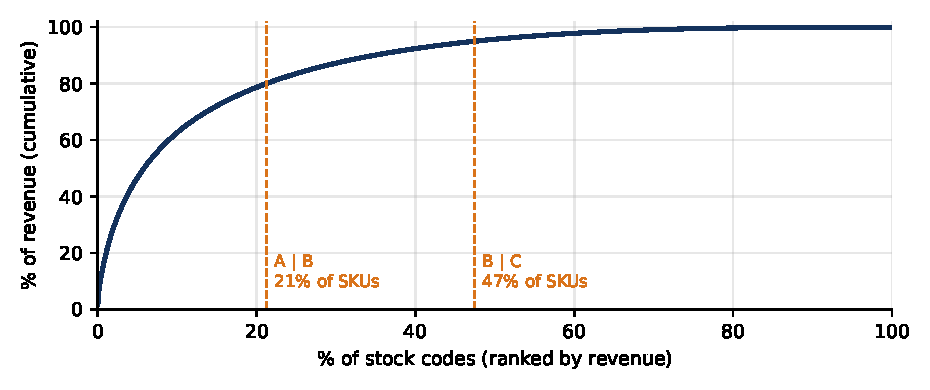
\includegraphics[width=0.86\linewidth]{../figs/lab1_pareto.pdf}
\caption{Pareto curve of revenue. 21\% of stock codes produce 80\% of revenue.}\end{figure}
\interp{1\,035 stock codes (21\% of the catalogue) make 80\% of revenue. The striking result is the XYZ column: only
65 items have steady demand. This is a gift wholesaler with a seasonal, fashion-driven range; most items are lumpy.
The CV is computed only between each item's first and last week of sales. Including the weeks before launch
would make new products look erratic when they are simply new.}

\begin{pitfall}{Measuring variability over the wrong window}
An item launched in October 2011 has 95 weeks of zeros before it. Its CV over the full period is huge, and an
automatic rule would classify it as ``Z, consider delisting'', which is exactly wrong for a new line. Segment on the
selling life, and treat new items separately.
\end{pitfall}

\step{Step 6: Export the demand table for Weeks 3 and 4}
\codeout{lab1_s6}{Weekly demand of A-class items with steady or variable demand.}
\interp{157 stock codes, 102 complete weeks each, in the long format (\texttt{unique\_id}, \texttt{ds}, \texttt{y})
that the forecasting libraries expect. The last, partial week of December 2011 is excluded: a four-day week would
look like a collapse in demand.}

\paragraph{So what (model answer)} \emph{Of \pounds20.1\,M in recorded sales, \pounds1.5\,M was cancelled and \pounds0.7\,M
was fees and adjustments, so demand planning must start from the cleaned table, not the raw export. One fifth of the
catalogue earns four fifths of revenue, but almost none of it sells steadily; replenishment rules that assume steady
demand will fail on most items. We will forecast the 157 A-class items that are steady enough to plan.}

% ------------------------------------------------------------------ EXERCISES
\section{Exercises}
\begin{enumerate}[label=\textbf{1.\arabic*},leftmargin=2.4em]
\item \emph{(Decision framing)} Write a full decision statement, with both error costs in XAF, for (a) the number of
cashiers on Saturday at Douala Akwa, (b) whether to hold a weekend promotion on cooking oil.
\item \emph{(KPI design)} A manager proposes ``average stock level'' as the inventory KPI for all stores. Give two
reasons it is a poor KPI and propose a pair of KPIs that cannot be gamed together.
\item \emph{(Calculation)} A line has OEE 72\%, availability 88\% and quality 97\%. What is its performance rate? Which
of the three factors would you investigate first, and why?
\item \emph{(SQL)} Using the \texttt{flagged} view, find the ten stock codes with the highest cancellation rate by value
among items with at least \pounds5\,000 of gross sales. What could explain the top three?
\item \emph{(SQL, grain)} Compute revenue per country two ways: summing line values, and joining an invoice-level
table to a country table after aggregating. Show a query that \emph{wrongly} double-counts and explain the fan-out.
\item \emph{(Mboa)} Load \texttt{data/sales.csv}. Write the five cleaning rules needed (duplicates, store-code case,
negative units, keying errors, missing units) as a single function that returns the cleaned table \emph{and} an audit
table of rows affected per rule. Which rule changes total units the most?
\item \emph{(Judgement)} Re-run Step 5 after removing the 33\,665 repeated lines. Does any item change ABC class? Write
three sentences to a manager on whether the decision matters.
\end{enumerate}

\section{Take-home assignment 1}
\begin{enumerate}[nosep]
\item Build a one-page Looker Studio dashboard for the Online Retail II sales director: monthly gross sales,
cancellation rate and average order value with year-on-year comparison, and the top 15 A-items. Every KPI must show its
definition. Share it read-only.
\item Write a 250-word memo: what the director should worry about, with numbers, and one action.
\item Push your notebook and a \texttt{requirements.txt} to your course GitHub repository.
\end{enumerate}
\paragraph{Capstone} Form teams of two. Bring two candidate decisions and datasets to Week 2 (see the Capstone chapter).
